\documentclass[aspectratio=169]{beamer}
\usetheme{Madrid}
\usecolortheme{default}
\setbeamertemplate{caption}{\raggedright\insertcaption\par}
\usepackage{fontspec}
\usepackage{graphicx}
\usepackage{hyperref}
\usepackage{booktabs}
\usepackage{xcolor}

\title[Chương 1: Tổng quan Học máy]{BỨC TRANH TỔNG QUAN VỀ HỌC MÁY \\ \vspace{0.5cm} \Large Chương 1 - Machine Learning}
\author{TS. Trần Thành Thắng}
\institute{Đại học Đông Á}
\date{\today}

\begin{document}

\begin{frame}
\titlepage
\end{frame}

\begin{frame}{Nội dung Chương trình}
\tableofcontents[hideallsubsections]
\end{frame}

\begin{frame}{Mục tiêu bài học}
\begin{itemize}
    \item Hiểu rõ định nghĩa và tầm quan trọng của Học máy (Machine Learning).
    \item Phân biệt các hệ thống Học máy (Có giám sát, Không giám sát, Bán giám sát, Học tăng cường).
    \item Nắm bắt quy trình phát triển một dự án Học máy thực tế.
    \item Nhận diện các thách thức chính (Overfitting, Underfitting, Chất lượng dữ liệu).
\end{itemize}
\end{frame}

\section{1. Khái quát \& Ứng dụng của Học máy}

\begin{frame}
\vfill\centering\LARGE\textbf{1. Khái quát \& Ứng dụng của Học máy}\vfill
\end{frame}

\begin{frame}{Đặt vấn đề: Bức tranh tổng quan}
\begin{itemize}
    \item Học máy không còn là khoa học viễn tưởng, nó hiện diện trong hàng tỷ thiết bị mỗi ngày.
    \item Từ thập niên 1990: Ứng dụng phổ biến đầu tiên là \textbf{Bộ lọc thư rác (Spam filter)}.
    \item Ngày nay: Lời nhắc bằng giọng nói, dịch tự động, tìm kiếm hình ảnh, đề xuất sản phẩm...
    \item Câu hỏi đặt ra: Một cỗ máy học hỏi điều gì và học như thế nào?
\end{itemize}
\end{frame}

\begin{frame}{Học máy là gì?}
\begin{block}{Định nghĩa 1 (Arthur Samuel, 1959)}
Học máy là lĩnh vực nghiên cứu cung cấp cho máy tính khả năng học hỏi mà không cần được lập trình rõ ràng.
\end{block}
\begin{block}{Định nghĩa 2 (Tom Mitchell, 1997)}
Một chương trình máy tính được cho là học từ kinh nghiệm \textbf{E} đối với một nhiệm vụ \textbf{T} và một thước đo hiệu suất \textbf{P}, nếu hiệu suất của nó trên T, được đo bằng P, cải thiện theo kinh nghiệm E.
\end{block}
\end{frame}

\begin{frame}{Cách tiếp cận truyền thống vs. Học máy}
\begin{columns}
\column{0.5\textwidth}
\begin{itemize}
    \item \textbf{Truyền thống:} Lập trình viên viết các quy tắc (rules) thủ công. Nếu vấn đề phức tạp, danh sách quy tắc sẽ dài bất tận và khó bảo trì.
\end{itemize}
\column{0.5\textwidth}
\begin{figure}
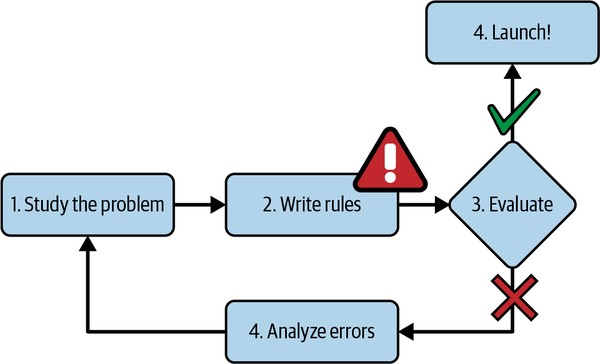
\includegraphics[width=\textwidth,height=0.7\textheight,keepaspectratio]{../machineLearningWeb/docs/../Figures/CH01/Hinh_1-1.jpg}
\caption{Hình 1-1. Cách tiếp cận truyền thống}
\end{figure}
\end{columns}
\end{frame}

\begin{frame}{Cách tiếp cận bằng Học máy}
\begin{columns}
\column{0.5\textwidth}
\begin{itemize}
    \item \textbf{Học máy:} Hệ thống tự động học các quy tắc từ dữ liệu (data) và đáp án (answers).
    \item Mã nguồn ngắn hơn, dễ bảo trì hơn và độ chính xác thường cao hơn rất nhiều.
\end{itemize}
\column{0.5\textwidth}
\begin{figure}
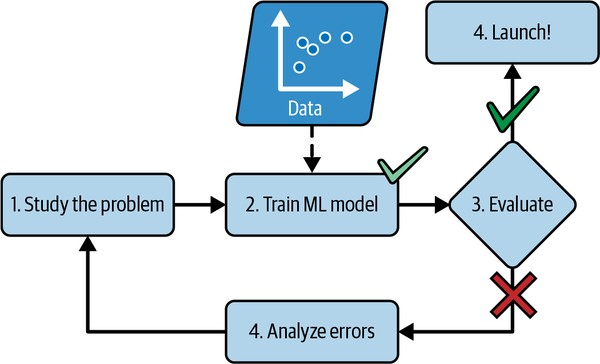
\includegraphics[width=\textwidth,height=0.7\textheight,keepaspectratio]{../machineLearningWeb/docs/../Figures/CH01/Hinh_1-2.jpg}
\caption{Hình 1-2. Phương pháp học máy}
\end{figure}
\end{columns}
\end{frame}

\begin{frame}{Tại sao sử dụng học máy?}
\begin{itemize}
    \item \textbf{Tự động thích ứng:} Khi dữ liệu thay đổi (ví dụ: spammer dùng từ lóng mới), mô hình học máy tự động cập nhật mà không cần lập trình lại.
    \item \textbf{Giải quyết bài toán phức tạp:} Những bài toán không có thuật toán truyền thống tối ưu (VD: nhận diện giọng nói).
    \item \textbf{Khám phá tri thức (Data Mining):} Tìm ra những quy luật ẩn giấu trong lượng dữ liệu khổng lồ.
\end{itemize}
\end{frame}

\begin{frame}{Tự động thích ứng với thay đổi}
\begin{figure}
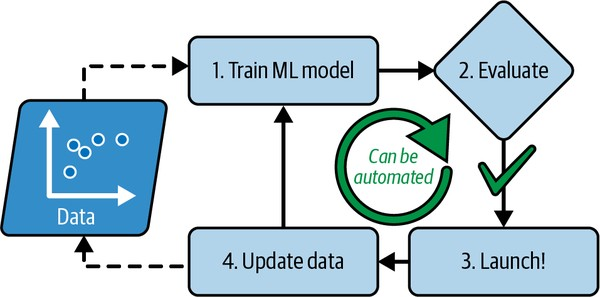
\includegraphics[width=0.7\textwidth,height=0.7\textheight,keepaspectratio]{../machineLearningWeb/docs/../Figures/CH01/Hinh_1-3.jpg}
\caption{Hình 1-3. Tự động thích ứng với dữ liệu mới}
\end{figure}
\end{frame}

\begin{frame}{Học máy giúp con người học hỏi}
\begin{figure}
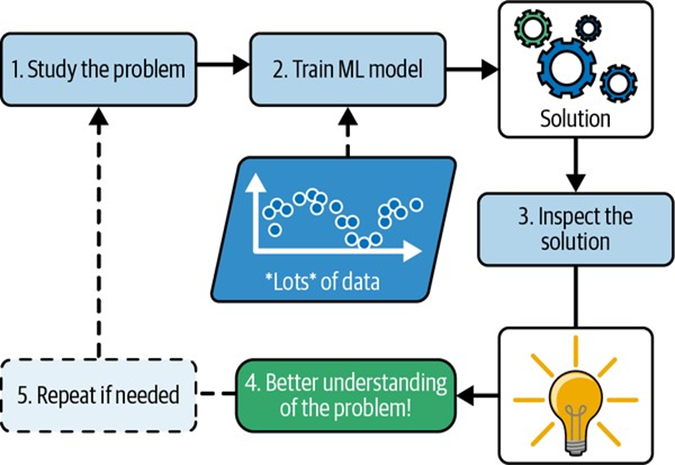
\includegraphics[width=0.7\textwidth,height=0.7\textheight,keepaspectratio]{../machineLearningWeb/docs/../Figures/CH01/Hinh_1-4.png}
\caption{Hình 1-4. Khai phá dữ liệu giúp con người tìm ra quy luật mới}
\end{figure}
\end{frame}

\begin{frame}{Ví dụ về các ứng dụng (1/2)}
\begin{itemize}
    \item \textbf{Phân tích hình ảnh sản phẩm:} Tự động phân loại sản phẩm trong quy trình sản xuất (Phân loại ảnh - CNN).
    \item \textbf{Phát hiện khối u não:} Trích xuất thông tin từ ảnh y tế (Phân đoạn ảnh - Semantic Segmentation).
    \item \textbf{Phân loại bài viết/tin tức:} Phân loại tự động các bài báo theo chủ đề (NLP - Phân loại văn bản).
\end{itemize}
\end{frame}

\begin{frame}{Ví dụ về các ứng dụng (2/2)}
\begin{itemize}
    \item \textbf{Đánh dấu nhận xét tiêu cực:} Phân tích cảm xúc từ phản hồi khách hàng ở diễn đàn.
    \item \textbf{Dự báo doanh thu:} Xây dựng mô hình dự báo tài chính dựa trên dữ liệu hiệu suất quá khứ (Hồi quy - Regression).
    \item \textbf{Phát hiện gian lận thẻ tín dụng:} Tìm ra các giao dịch bất thường (Phát hiện bất thường - Anomaly Detection).
\end{itemize}
\end{frame}

\section{2. Phân loại Hệ thống Học máy}

\begin{frame}
\vfill\centering\LARGE\textbf{2. Phân loại Hệ thống Học máy}\vfill
\end{frame}

\begin{frame}{Tiêu chí phân loại hệ thống học máy}
Có ba tiêu chí chính để phân loại:
\begin{enumerate}
    \item \textbf{Sự giám sát của con người:} Học có giám sát, Không giám sát, Bán giám sát, và Học tăng cường.
    \item \textbf{Khả năng học tăng dần:} Học trực tuyến (Online) vs Học theo lô (Batch).
    \item \textbf{Cách tổng quát hóa:} Học dựa trên thực thể (Instance-based) vs Học dựa trên mô hình (Model-based).
\end{enumerate}
\end{frame}

\begin{frame}{Học có giám sát (Supervised Learning)}
\begin{columns}
\column{0.5\textwidth}
\begin{itemize}
    \item Dữ liệu huấn luyện cung cấp cho thuật toán bao gồm các giải pháp mong muốn, được gọi là \textbf{nhãn (labels)}.
    \item Ví dụ điển hình: Bộ lọc thư rác (Spam filter).
\end{itemize}
\column{0.5\textwidth}
\begin{figure}
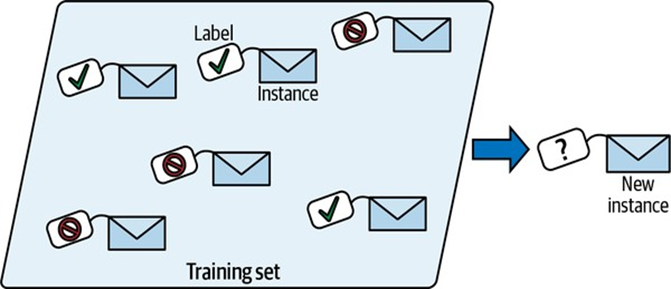
\includegraphics[width=\textwidth,height=0.6\textheight,keepaspectratio]{../machineLearningWeb/docs/../Figures/CH01/Hinh_1-5.png}
\caption{Hình 1-5. Bộ dữ liệu có nhãn cho học có giám sát}
\end{figure}
\end{columns}
\end{frame}

\begin{frame}{Phân loại (Classification) vs Hồi quy (Regression)}
\begin{columns}
\column{0.5\textwidth}
\begin{itemize}
    \item \textbf{Phân loại:} Dự đoán danh mục/lớp (Rác/Không rác).
    \item \textbf{Hồi quy:} Dự đoán một giá trị mục tiêu (giá xe hơi) dựa trên các tập đặc trưng (đã đi bao nhiêu km, nhãn hiệu...).
\end{itemize}
\column{0.5\textwidth}
\begin{figure}
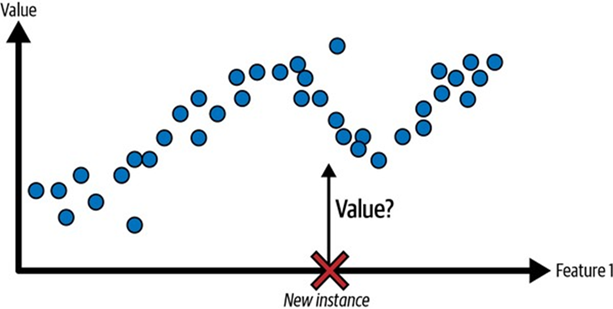
\includegraphics[width=\textwidth,height=0.6\textheight,keepaspectratio]{../machineLearningWeb/docs/../Figures/CH01/Hinh_1-6.png}
\caption{Hình 1-6. Bài toán hồi quy (Regression)}
\end{figure}
\end{columns}
\end{frame}

\begin{frame}{Học không giám sát (Unsupervised Learning)}
\begin{columns}
\column{0.5\textwidth}
\begin{itemize}
    \item Dữ liệu huấn luyện \textbf{không được gắn nhãn}. Hệ thống cố gắng học mà không cần người hướng dẫn.
    \item Dùng để tìm kiếm cấu trúc ẩn trong dữ liệu.
\end{itemize}
\column{0.5\textwidth}
\begin{figure}
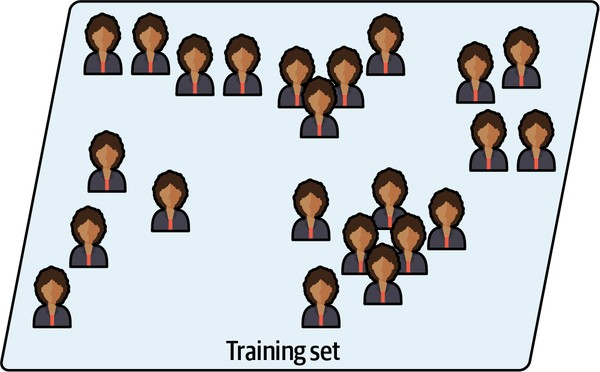
\includegraphics[width=\textwidth,height=0.6\textheight,keepaspectratio]{../machineLearningWeb/docs/../Figures/CH01/Hinh_1-7.jpg}
\caption{Hình 1-7. Tập dữ liệu không gán nhãn}
\end{figure}
\end{columns}
\end{frame}

\begin{frame}{Phân cụm (Clustering)}
\begin{columns}
\column{0.5\textwidth}
\begin{itemize}
    \item Tự động nhóm dữ liệu thành các cụm có chung đặc điểm.
    \item \textbf{Ví dụ:} Gom cụm khách hàng trên trang web thành các phân khúc để chạy chiến dịch quảng cáo mục tiêu.
\end{itemize}
\column{0.5\textwidth}
\begin{figure}
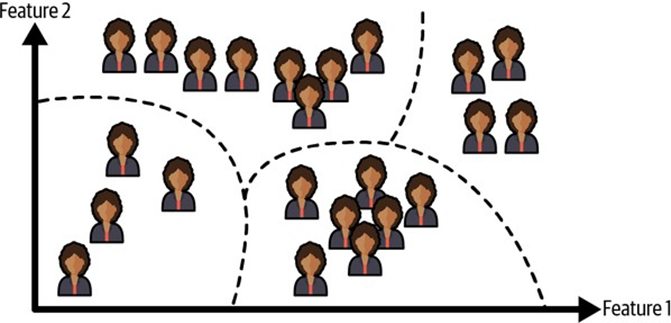
\includegraphics[width=\textwidth,height=0.6\textheight,keepaspectratio]{../machineLearningWeb/docs/../Figures/CH01/Hinh_1-8.png}
\caption{Hình 1-8. Phân cụm (Clustering)}
\end{figure}
\end{columns}
\end{frame}

\begin{frame}{Giảm chiều dữ liệu (Dimensionality Reduction)}
\begin{columns}
\column{0.5\textwidth}
\begin{itemize}
    \item Đơn giản hóa dữ liệu mà không làm mất quá nhiều thông tin.
    \item \textbf{Trích xuất đặc trưng:} Kết hợp nhiều đặc trưng tương quan thành 1 đặc trưng mới.
\end{itemize}
\column{0.5\textwidth}
\begin{figure}
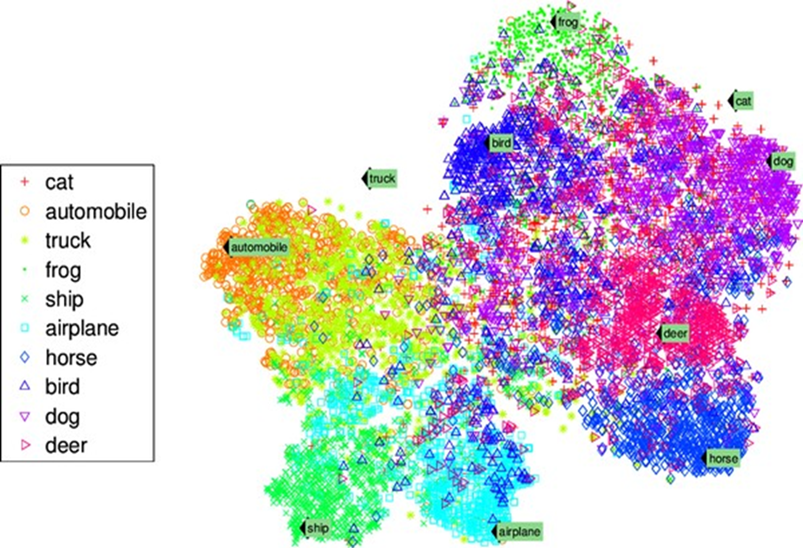
\includegraphics[width=\textwidth,height=0.6\textheight,keepaspectratio]{../machineLearningWeb/docs/../Figures/CH01/Hinh_1-9.png}
\caption{Hình 1-9. Giảm chiều (từ 3D xuống 2D)}
\end{figure}
\end{columns}
\end{frame}

\begin{frame}{Phát hiện bất thường (Anomaly Detection) \& Luật kết hợp}
\begin{itemize}
    \item Phát hiện gian lận thẻ tín dụng, lỗi sản xuất, xóa ngoại lai trước khi huấn luyện mô hình.
    \item \textbf{Luật kết hợp (Association Rule):} Tìm kiếm mối liên hệ (VD: Khách mua bỉm thường mua thêm bia).
\end{itemize}
\end{frame}

\begin{frame}{Minh họa: Bất thường \& Luật kết hợp}
\begin{figure}
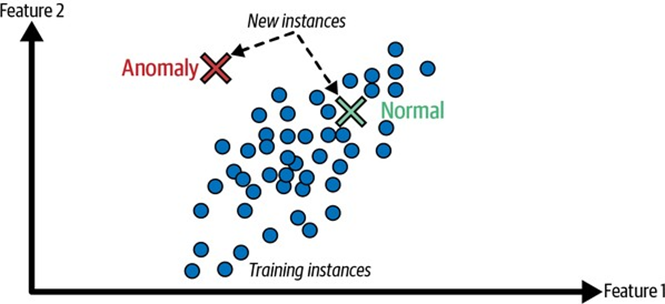
\includegraphics[width=0.7\textwidth,height=0.65\textheight,keepaspectratio]{../machineLearningWeb/docs/../Figures/CH01/Hinh_1-10.png}
\caption{Hình 1-10. Phát hiện bất thường}
\end{figure}
\end{frame}

\begin{frame}{Học bán giám sát (Semi-supervised Learning)}
\begin{columns}
\column{0.5\textwidth}
\begin{itemize}
    \item Dữ liệu bao gồm rất nhiều mẫu chưa gán nhãn, và chỉ có một số ít mẫu được gán nhãn.
    \item Phổ biến trong nhận diện ảnh (Google Photos). Thuật toán (như DBNs) gộp các đặc điểm chung trước khi cần con người định danh 1 người cụ thể.
\end{itemize}
\column{0.5\textwidth}
\begin{figure}
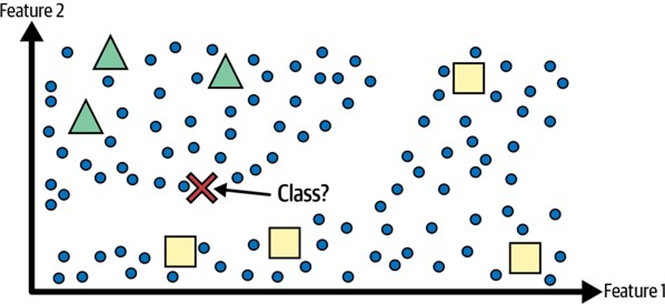
\includegraphics[width=\textwidth,height=0.6\textheight,keepaspectratio]{../machineLearningWeb/docs/../Figures/CH01/Hinh_1-11.png}
\caption{Hình 1-11. Học bán giám sát}
\end{figure}
\end{columns}
\end{frame}

\begin{frame}{Học tự giám sát (Self-supervised Learning)}
\begin{columns}
\column{0.5\textwidth}
\begin{itemize}
    \item Tạo ra tập dữ liệu có nhãn từ dữ liệu hoàn toàn không nhãn.
    \item Ví dụ: Che một phần hình ảnh và yêu cầu mô hình khôi phục phần bị che.
    \item Thường được dùng để tạo ra một mô hình cơ sở, sau đó tinh chỉnh (fine-tune) cho tác vụ cụ thể.
\end{itemize}
\column{0.5\textwidth}
\begin{figure}
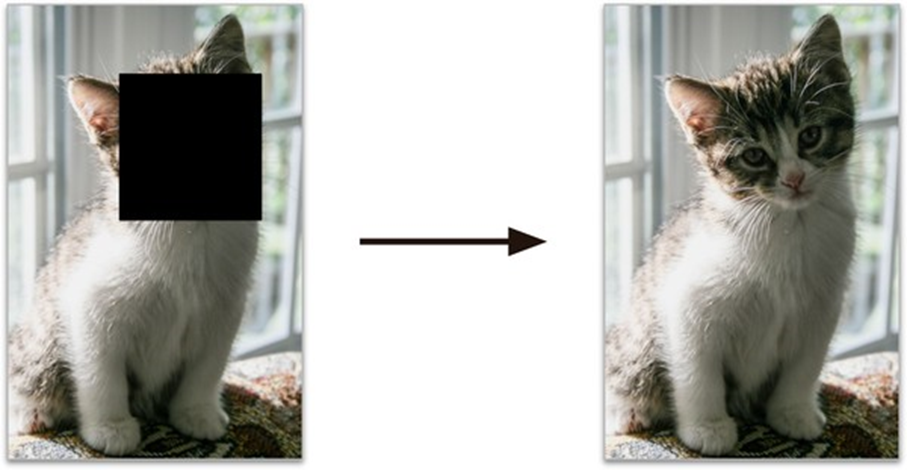
\includegraphics[width=\textwidth,height=0.6\textheight,keepaspectratio]{../machineLearningWeb/docs/../Figures/CH01/Hinh_1-12.png}
\caption{Hình 1-12. Ví dụ học tự giám sát}
\end{figure}
\end{columns}
\end{frame}

\begin{frame}{Học tăng cường (Reinforcement Learning)}
\begin{columns}
\column{0.5\textwidth}
\begin{itemize}
    \item Hệ thống (Agent) quan sát môi trường, thực hiện hành động và nhận về phần thưởng/hình phạt.
    \item Nó phải tự học ra chính sách (Policy) tốt nhất để tối đa hóa phần thưởng. (Ví dụ: AlphaGo).
\end{itemize}
\column{0.5\textwidth}
\begin{figure}
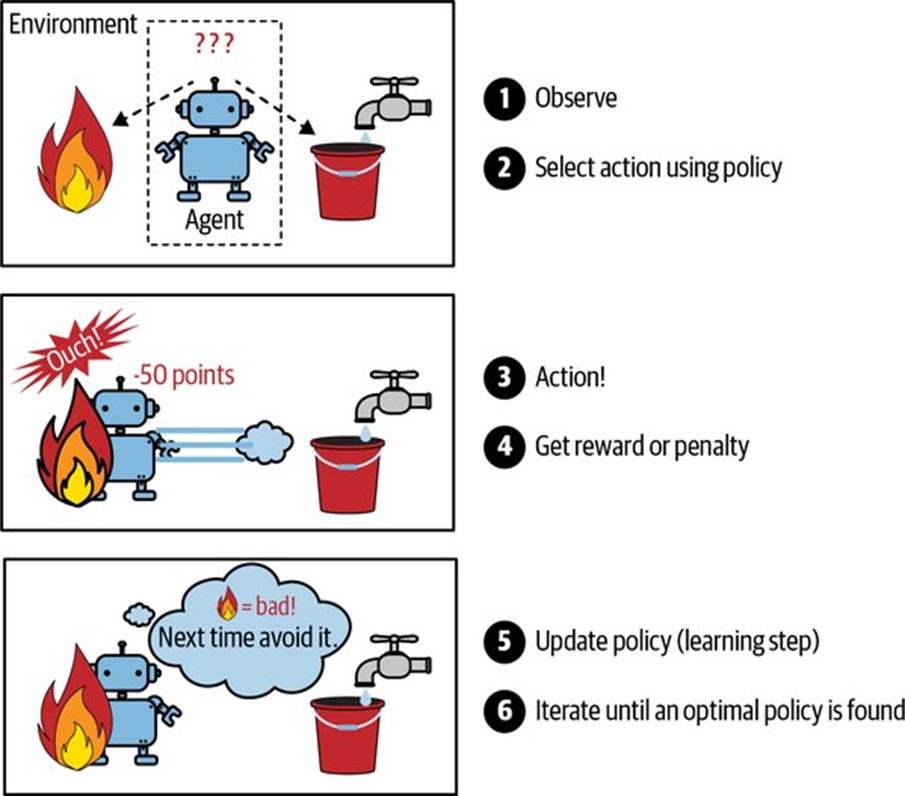
\includegraphics[width=\textwidth,height=0.6\textheight,keepaspectratio]{../machineLearningWeb/docs/../Figures/CH01/Hinh_1-13.png}
\caption{Hình 1-13. Cơ chế Học tăng cường}
\end{figure}
\end{columns}
\end{frame}

\begin{frame}{Học theo lô vs Học trực tuyến (Batch vs Online)}
\begin{itemize}
    \item \textbf{Học theo lô (Batch):} Huấn luyện một lần với toàn bộ dữ liệu. Tốn thời gian, tài nguyên. Nếu có dữ liệu mới phải huấn luyện lại từ đầu.
    \item \textbf{Học trực tuyến (Online):} Huấn luyện theo từng phần dữ liệu nhỏ (mini-batches). Phù hợp với luồng dữ liệu liên tục (Chứng khoán, Thời tiết).
\end{itemize}
\end{frame}

\begin{frame}{Minh họa: Học trực tuyến}
\begin{figure}
\centering
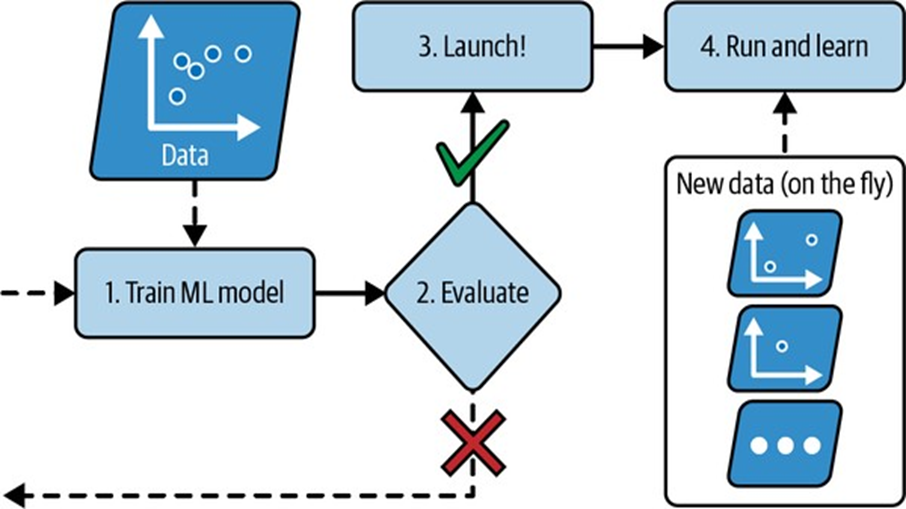
\includegraphics[width=0.8\textwidth,height=0.7\textheight,keepaspectratio]{../machineLearningWeb/docs/../Figures/CH01/Hinh_1-14.png}
\caption{Hình 1-14. Học trực tuyến}
\end{figure}
\end{frame}

\begin{frame}{Học với tập dữ liệu khổng lồ (Out-of-core)}
\begin{figure}
\centering
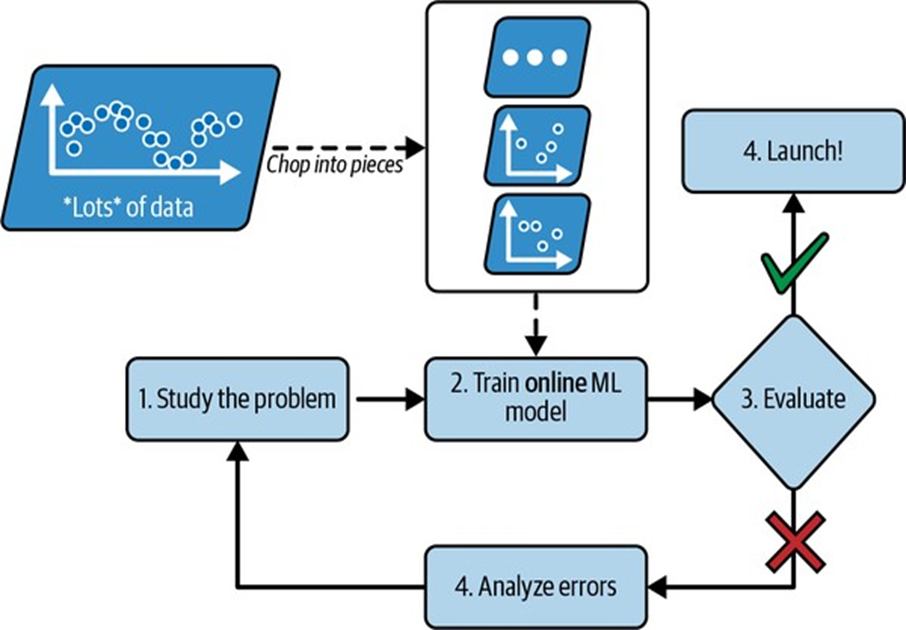
\includegraphics[width=0.8\textwidth,height=0.7\textheight,keepaspectratio]{../machineLearningWeb/docs/../Figures/CH01/Hinh_1-15.png}
\caption{Hình 1-15. Học với tập dữ liệu khổng lồ (Out-of-core)}
\end{figure}
\end{frame}

\begin{frame}{Học dựa trên thực thể (Instance-based Learning)}
\begin{columns}
\column{0.5\textwidth}
\begin{itemize}
    \item Hệ thống học bằng cách \textbf{ghi nhớ} các ví dụ.
    \item Khi có mẫu mới, nó so sánh độ tương đồng (Ví dụ: tính số lượng từ giống nhau) với các mẫu đã biết để đưa ra quyết định.
\end{itemize}
\column{0.5\textwidth}
\begin{figure}
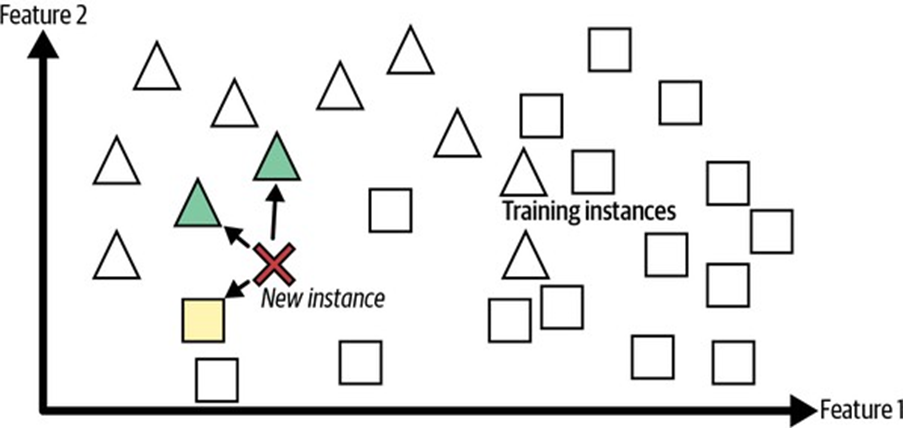
\includegraphics[width=\textwidth,height=0.6\textheight,keepaspectratio]{../machineLearningWeb/docs/../Figures/CH01/Hinh_1-16.png}
\caption{Hình 1-16. Học dựa trên thực thể}
\end{figure}
\end{columns}
\end{frame}

\begin{frame}{Học dựa trên mô hình (Model-based Learning)}
\begin{columns}
\column{0.5\textwidth}
\begin{itemize}
    \item Xây dựng một \textbf{mô hình} từ các ví dụ, sau đó dùng mô hình đó để dự đoán.
    \item \textbf{Ví dụ:} Tìm ra hàm tuyến tính $y = ax + b$ phản ánh mối quan hệ giữa "GDP bình quân đầu người" và "Mức độ hài lòng với cuộc sống".
\end{itemize}
\column{0.5\textwidth}
\begin{figure}
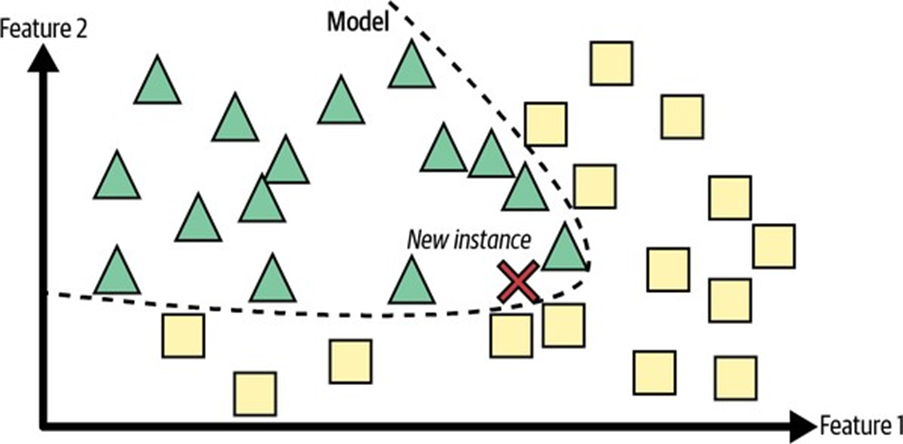
\includegraphics[width=\textwidth,height=0.6\textheight,keepaspectratio]{../machineLearningWeb/docs/../Figures/CH01/Hinh_1-17.png}
\caption{Hình 1-17. Học dựa trên mô hình}
\end{figure}
\end{columns}
\end{frame}

\begin{frame}{Minh họa: Biểu đồ phân tán \& Mô hình phù hợp nhất}
\begin{columns}
\column{0.5\textwidth}
\begin{figure}
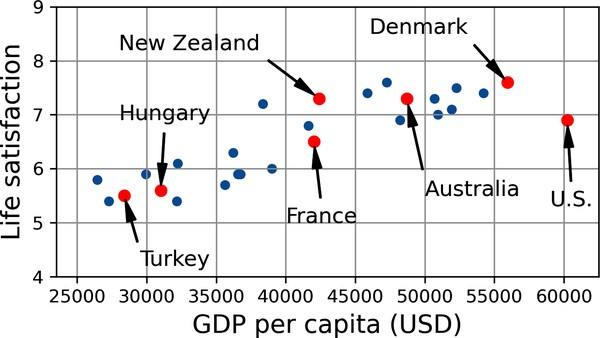
\includegraphics[width=\textwidth,height=0.55\textheight,keepaspectratio]{../machineLearningWeb/docs/../Figures/CH01/Hinh_1-18.jpg}
\caption{Hình 1-18. Biểu đồ phân tán (xu hướng)}
\end{figure}
\column{0.5\textwidth}
\begin{figure}
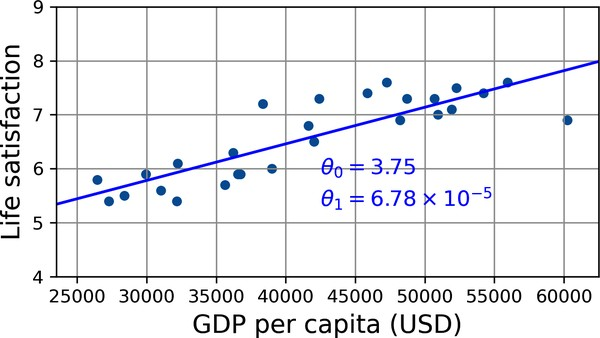
\includegraphics[width=\textwidth,height=0.55\textheight,keepaspectratio]{../machineLearningWeb/docs/../Figures/CH01/Hinh_1-20.jpg}
\caption{Hình 1-20. Mô hình tuyến tính phù hợp nhất}
\end{figure}
\end{columns}
\begin{itemize}
    \item Bằng cách định nghĩa \textbf{hàm chi phí (Cost Function)} và tối thiểu hóa nó, hệ thống sẽ tìm ra tham số tốt nhất cho mô hình.
\end{itemize}
\end{frame}

\section{3. Thách thức, Kiểm thử \& Xác thực}

\begin{frame}
\vfill\centering\LARGE\textbf{3. Thách thức, Kiểm thử \& Xác thực}\vfill
\end{frame}

\begin{frame}{Những thách thức chính của học máy}
Mô hình "Dữ liệu tồi" (Bad Data) hoặc "Thuật toán tồi" (Bad Algorithm):
\begin{itemize}
    \item Dữ liệu huấn luyện không đủ lớn.
    \item Dữ liệu huấn luyện không đại diện.
    \item Dữ liệu chất lượng kém (nhiễu, ngoại lai).
    \item Đặc trưng không liên quan (Garbage in, garbage out).
    \item Khớp quá mức (Overfitting) dữ liệu huấn luyện.
    \item Chưa khớp (Underfitting) dữ liệu huấn luyện.
\end{itemize}
\end{frame}

\begin{frame}{Dữ liệu huấn luyện không đủ (Dữ liệu tồi)}
\begin{itemize}
    \item Máy tính cần hàng nghìn, thậm chí hàng triệu ví dụ mới có thể học được các tác vụ phức tạp (nhận dạng hình ảnh, xử lý ngôn ngữ).
    \item Hiệu quả dữ liệu đôi khi còn quan trọng hơn cả thuật toán tinh vi.
\end{itemize}
\begin{figure}
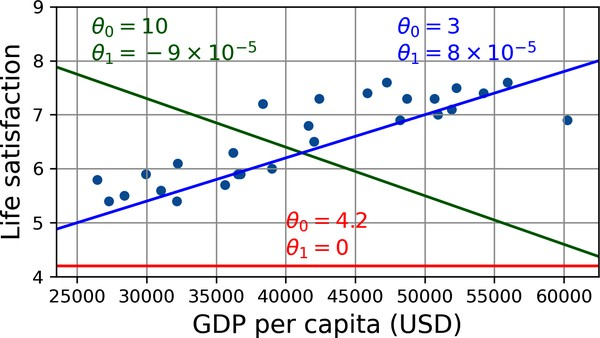
\includegraphics[width=0.7\textwidth,height=0.5\textheight,keepaspectratio]{../machineLearningWeb/docs/../Figures/CH01/Hinh_1-19.jpg}
\caption{Hình 1-19. Tầm quan trọng của khối lượng dữ liệu (Nghiên cứu của Microsoft)}
\end{figure}
\end{frame}

\begin{frame}{Dữ liệu huấn luyện không đại diện}
\begin{columns}
\column{0.5\textwidth}
\begin{itemize}
    \item Để dự đoán tốt, dữ liệu phải đại diện cho các trường hợp mới mà mô hình sẽ gặp.
    \item Nếu dữ liệu bị thiên lệch, mô hình sẽ sai lầm (Lỗi lấy mẫu - Sampling bias).
\end{itemize}
\column{0.5\textwidth}
\begin{figure}
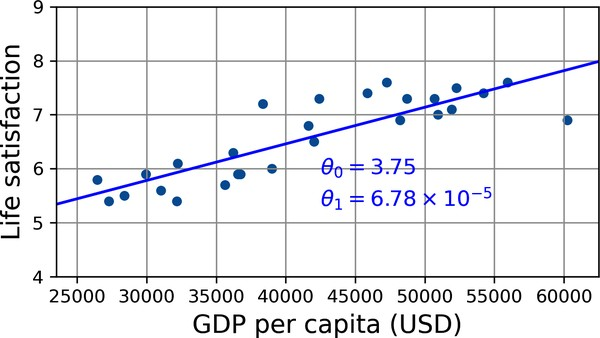
\includegraphics[width=\textwidth,height=0.6\textheight,keepaspectratio]{../machineLearningWeb/docs/../Figures/CH01/Hinh_1-20.jpg}
\caption{Hình 1-20. Lỗi dự báo nếu bỏ qua một số quốc gia khỏi tập huấn luyện}
\end{figure}
\end{columns}
\end{frame}

\begin{frame}{Dữ liệu chất lượng kém}
\begin{itemize}
    \item \textbf{Chất lượng kém:} Nhiều lỗi, ngoại lai (outliers), giá trị nhiễu. Cần tốn thời gian làm sạch (Data Cleaning).
    \item Hầu hết các Data Scientist dành phần lớn thời gian cho việc làm sạch dữ liệu.
\end{itemize}
\end{frame}

\begin{frame}{Đặc trưng không liên quan}
\begin{itemize}
    \item \textbf{Đặc trưng không liên quan:} Thuật toán học máy chỉ tốt khi thông tin nạp vào là hữu ích (Garbage In, Garbage Out).
    \item \textbf{Kỹ thuật đặc trưng (Feature Engineering):} 
    \begin{itemize}
        \item Lựa chọn đặc trưng (Feature Selection).
        \item Trích xuất đặc trưng (Feature Extraction).
        \item Tạo đặc trưng mới.
    \end{itemize}
\end{itemize}
\end{frame}

\begin{frame}{Overfitting (Khớp quá mức)}
\begin{columns}
\column{0.5\textwidth}
\begin{itemize}
    \item Mô hình hoạt động tuyệt vời trên tập huấn luyện nhưng dự đoán cực kém với dữ liệu mới.
    \item Xảy ra khi mô hình quá phức tạp so với lượng dữ liệu, hoặc dữ liệu quá nhiễu.
    \item \textbf{Khắc phục:} Đơn giản hóa mô hình, thêm dữ liệu, giảm nhiễu, hoặc Dừng sớm.
\end{itemize}
\column{0.5\textwidth}
\begin{figure}
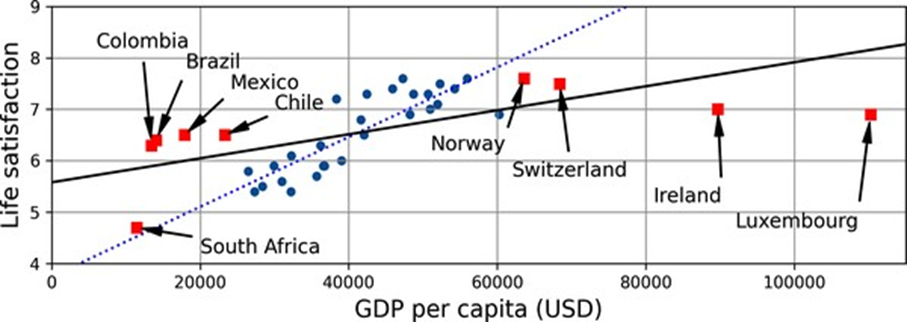
\includegraphics[width=\textwidth,height=0.6\textheight,keepaspectratio]{../machineLearningWeb/docs/../Figures/CH01/Hinh_1-22.png}
\caption{Hình 1-22. Khớp quá mức (Overfitting) với mô hình đa thức phức tạp}
\end{figure}
\end{columns}
\end{frame}

\begin{frame}{Điều chuẩn (Regularization)}
\begin{columns}
\column{0.5\textwidth}
\begin{itemize}
    \item Phương pháp ràng buộc mô hình để làm nó đơn giản hơn và giảm rủi ro Overfitting.
    \item Hình bên cho thấy hiệu quả của Regularization: mô hình bớt cong vẹo và ít phụ thuộc vào nhiễu hơn.
\end{itemize}
\column{0.5\textwidth}
\begin{figure}
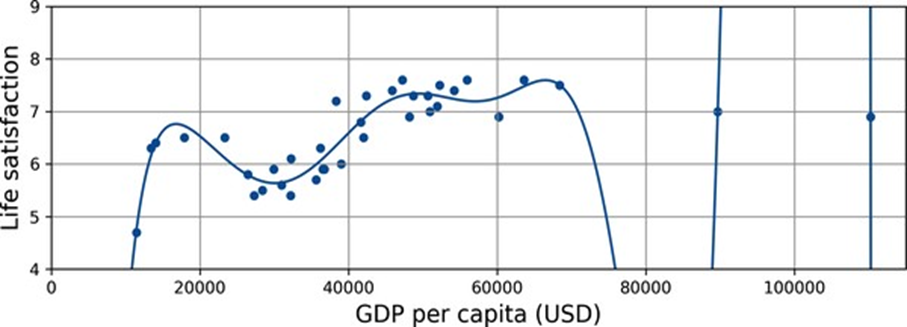
\includegraphics[width=\textwidth,height=0.6\textheight,keepaspectratio]{../machineLearningWeb/docs/../Figures/CH01/Hinh_1-23.png}
\caption{Hình 1-23. Hiệu ứng của việc điều chuẩn để giảm Overfitting}
\end{figure}
\end{columns}
\end{frame}

\begin{frame}{Underfitting (Chưa khớp)}
\begin{columns}
\column{0.5\textwidth}
\begin{itemize}
    \item Mô hình quá đơn giản, không đủ khả năng học các cấu trúc ẩn bên trong dữ liệu (Ví dụ: dùng mô hình tuyến tính cho dữ liệu phi tuyến).
    \item \textbf{Khắc phục:} Chọn mô hình phức tạp hơn, cung cấp đặc trưng tốt hơn, hoặc nới lỏng các ràng buộc (giảm Regularization).
\end{itemize}
\column{0.5\textwidth}
\begin{figure}
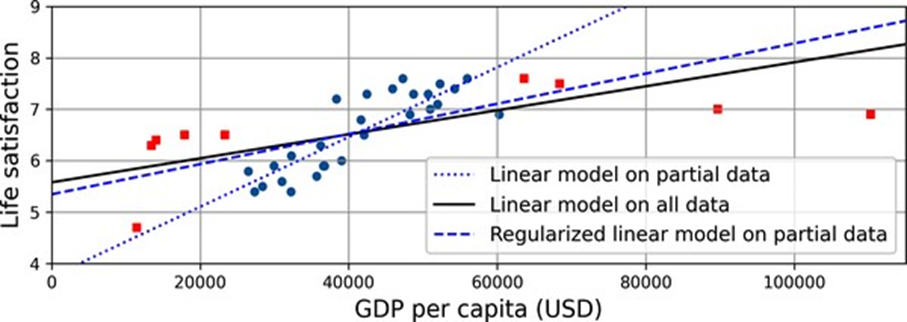
\includegraphics[width=\textwidth,height=0.6\textheight,keepaspectratio]{../machineLearningWeb/docs/../Figures/CH01/Hinh_1-24.png}
\caption{Hình 1-24. Underfitting - Đường dự đoán bị lệch khỏi xu thế thực}
\end{figure}
\end{columns}
\end{frame}

\begin{frame}{Kiểm thử và xác thực (Testing and Validating)}
\begin{itemize}
    \item Để biết mô hình có tốt không, không thể chỉ đánh giá trên tập huấn luyện (vì có thể bị Overfitting).
    \item \textbf{Chia dữ liệu:} Thường chia thành $80\%$ \textbf{Tập huấn luyện (Training Set)} và $20\%$ \textbf{Tập kiểm thử (Test Set)}.
    \item \textbf{Lỗi tổng quát hóa (Generalization Error):} Tỉ lệ lỗi trên tập kiểm thử đại diện cho khả năng ứng dụng thực tế.
\end{itemize}
\end{frame}

\begin{frame}{Tinh chỉnh mô hình và Tập xác thực (Validation Set)}
\begin{itemize}
    \item Nếu bạn dùng Test Set để tinh chỉnh tham số (Hyperparameters), mô hình sẽ "học vẹt" Test Set $\Rightarrow$ Lỗi dự báo khi thực tế đưa vào vẫn cao.
    \item \textbf{Giải pháp:} Tách riêng một phần dữ liệu huấn luyện thành \textbf{Tập xác thực (Validation Set)}.
    \item \textbf{Cross-Validation:} Giúp tối đa hóa hiệu năng khi dữ liệu bị hạn chế.
\end{itemize}
\begin{figure}
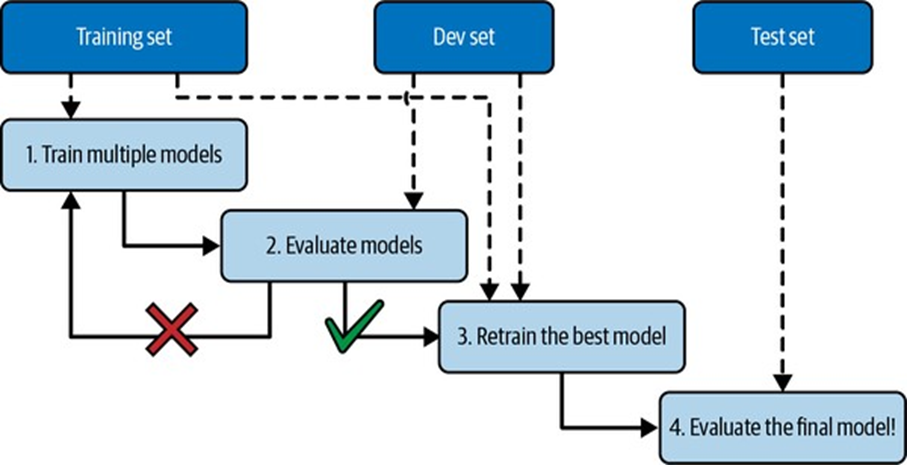
\includegraphics[width=0.6\textwidth,height=0.4\textheight,keepaspectratio]{../machineLearningWeb/docs/../Figures/CH01/Hinh_1-25.png}
\caption{Hình 1-25. Kỹ thuật Cross-Validation}
\end{figure}
\end{frame}

\begin{frame}{Sự không khớp dữ liệu (Data Mismatch) \& Tập train-dev}
\begin{columns}
\column{0.5\textwidth}
\begin{itemize}
    \item Xảy ra khi dữ liệu huấn luyện dồi dào nhưng không đại diện hoàn toàn cho thực tế (Ví dụ: ảnh tải từ web vs ảnh chụp thực tế bằng di động).
    \item \textbf{Giải pháp:} Giữ lại một phần dữ liệu huấn luyện thành \textbf{Tập train-dev}.
    \item Giúp phân biệt rõ mô hình bị \textbf{Overfitting} hay bị \textbf{Data Mismatch}.
\end{itemize}
\column{0.5\textwidth}
\begin{figure}
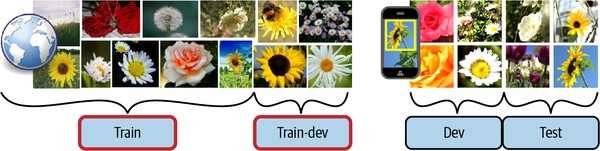
\includegraphics[width=\textwidth,height=0.6\textheight,keepaspectratio]{../machineLearningWeb/docs/../Figures/CH01/Hinh_1-26.jpg}
\caption{Hình 1-26. Sử dụng tập train-dev để đánh giá}
\end{figure}
\end{columns}
\end{frame}

\begin{frame}{Không có bữa trưa miễn phí (No Free Lunch)}
\begin{itemize}
    \item "Không có mô hình học máy nào luôn luôn tốt nhất cho mọi loại dữ liệu" (Định lý Wolpert, 1996).
    \item Nếu bạn hoàn toàn không biết gì về dữ liệu, không có lý do gì để ưu tiên mô hình này hơn mô hình khác.
    \item Đơn giản hóa có nghĩa là mô hình phải loại bỏ các chi tiết thừa thãi.
    \item Cần đưa ra một số giả định hợp lý và thử nghiệm nhiều mô hình khác nhau.
\end{itemize}
\end{frame}

\begin{frame}{Tổng kết Chương 1}
\begin{itemize}
    \item Học máy là việc làm cho máy tính thực hiện công việc dựa trên kinh nghiệm từ dữ liệu.
    \item Bao gồm nhiều loại (Supervised, Unsupervised, Reinforcement, Batch, Online, Instance, Model).
    \item Phụ thuộc vào chất lượng \& số lượng dữ liệu.
    \item Luôn phải cân bằng giữa Overfitting và Underfitting.
    \item Phải đánh giá nghiêm ngặt bằng tập Train/Validation/Test.
\end{itemize}
\end{frame}

\end{document}
